\chapter{Theory}

In this chapter, we give a theoretical introduction to the topic dealt with in this thesis. The ultimate goal of this chapter is to introduce and describe a analytical model for subsurface scattering. First, we will give a brief introduction to what light is, and how we physically describe it. Secondly, we will introduce the basic radiometric quantities that will be used throughout the chapter. Then, we will describe how this quantities are related and can be used to describe light-material interaction, using reflectance functions, of which BSSRDF functions are a special case. Finally, we will introduce subsurface scattering and the diffusion approximation, concluding with a description of two BSSRDF functions actually used to describe it, by \cite{Jensen:2001:PMS:383259.383319} and \cite{IMM2013-06646}.

\section{Light and Radiometry}
Light is a form of electromagnetic radiation, a sinusoidal wave that propagates through space. Usually by light we generically refer to \emph{visible light}, the small part of the electromagnetic spectrum the human eye is sensible to. This small window is between 380 nm of the infrared and 770 nm of the ultraviolet, but the precise boundaries vary according to the environment and the observer. Instead explicitly noted, we will use the terms light and visible light interchangeably.

The study of light is usually referred as optics. In computer aided image synthesis, we are interested in representing faithfully how visible light propagates though the scene and how interacts with materials. In addition, we are interested on effects that are noticeable at human scales. So, we are interested for example in subsurface scattering, absorption and emission but not in phenomena like diffraction, interference and quantum effects, that happen on a microscopic scale. 

\begin{figure}[!ht]
\centering
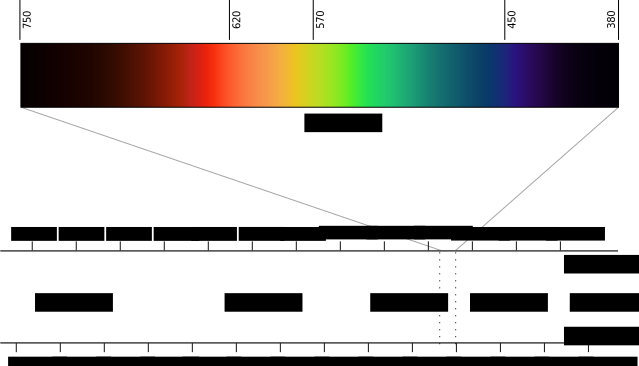
\includegraphics[width=1.0\textwidth]{images/spectrum.pdf}
\caption{The electromagnetic spectrum.}
\label{fig:spectrum}
\end{figure}

The study of the measurement of electromagnetic radiation is called \emph{radiometry}. The energy of light, like all the others forms of energy, is measured in \emph{Joules (J)}, and its power in \emph{Watts (W)}. \emph{Photometry}, on the other hand, measures electromagnetic radiation as it is perceived from the human eye, and limits itself only to the visible spectrum, while radiometry spans all of it. The quantities for energy and power are called respectively \emph{talbot (Cd $\cdot$ s)} and \emph{candela (Cd)}. 

In image synthesis radiometry, is employed, as its quantities are universal and can be easily converted to the photometric ones when necessary. The most important radiometric quantities used in computer graphics are radiant energy, radiant power, radiance, irradiance and intensity.

\section{Radiometric quantities}

\subsection{Radiant flux}
The radiant flux, also known as radiant power, is the most basic quantity in radiometry. It is usually indicated with the letter $\Phi$ and it is measured in joules per seconds ($J/s$) or Watts ($W$). The quantity indicates how much power the light irradiates per unit time. Given its nature, the radiant flux is constant irregardless of the distance from the light source.

\subsection{Radiant energy}
Radiant energy, usually indicated as $Q$, is the energy that the light carries in a certain amount of time. Like all the other SI units for energy, it is measured in joules ($J$). Radiant energy is usually obtained integrating the radiant flux along time:

$$
Q = \int_{\Delta T} \Phi \; dt
$$

Due to the dual nature of the light, the energy carried by the light can be derived both considering the flux of photons as particles, or considering light as a wave. We will not dig further into the topic, because for rendering purposes is not important how we characterize light.

\subsection{Irradiance}

Irradiance, usually defined as $E$, is the radiometric unit that measures the radiant flux per unit area \emph{falling} on a surface. It is measuerd in Watts per square meter ($W/m^2$). It is obtained by further deriving the differential of the radiant flux by the differential area:

$$
E = \frac{d\Phi}{dA}
$$

Irradiance is usually the term using for the incoming power. The converse, i.e. the irradiance leaving a surface, it is usually referred as radiant exitance or radiosity, and indicated with the letter $B$.
 
\subsection{Intensity}
Intensity is often a misused term in the physics community, as it is used for a lot of different measures. Depending on the community, intensity may refer to irradiance or even to radiance (see following section). We will refer to intensity as it is generally interpreted by the optics community, i.e. radiant intensity. It is defined as the differential radiant flux per differential solid angle:

$$
I(\vec{\omega}) = \frac{d \Phi}{d \omega}
$$

Intensity is measured in Watts / steradian ($W/sr$) and it is indicated with the letter $I$.

\subsection{Radiance}
Radiance is the most important quantity in image synthesis. It is defined precisely as the differential flux per solid angle per projected surface area, and it is measured in Watt per steradian per square meter ($W / (sr \cdot m^2)$).

$$
L(\vec{\omega}) = \frac{d^2 \Phi}{d\omega dA \cos \theta}
$$

Where $\theta$ is the angle between the surface normal and the incoming ray of light. Radiance is important in image synthesis because it is the natural quantity to associate with a ray of light (as it remains constant) and because is the quantity the human eye is actually sensible to. For a discussion on why radiance is related to the sensitivity of sensors and the human eye, see X.

All the other radiometric quantities can be derived from radiance:

\begin{equation*}
\begin{split}
E &= \int_{\Omega} L_i(\vec{\omega}) \cos\theta \; d\omega \\
I(\vec{\omega}) &= \int_A L(\vec{\omega}) \cos\theta \; dA \\
\Phi &= \int_A \int_{\Omega} L(\vec{\omega}) \cos\theta \; d\omega dA
\end{split}
\end{equation*}

\begin{itemize}
	\item Radiometric quantities

		\begin{itemize}
			\item 	\item Radiant Energy
			\item Radiant Power
			\item Radiance (L)
			\item Irradiance and Radiosity (E/B)
			\item Intensity (I)

\end{itemize}
	\item Reflectance Functions
	
	\begin{itemize}
		\item BRDFs and reflectance
		\item The rendering equation
		\item Mirror reflections, diffuse reflections and glossy reflections
		\item BSSRDFs functions
   	\item Fresnel equations

	\end{itemize}
	
	\item Light transport in volumes
	\item Scattering parameters: emission, absorption, scattering and phase functions
	
	\item Jensen's Dipole - diffusion approximation 
	\item Jeppe's Dipole
	
\end{itemize}
